\chapter{Aplikacja webowa do powiększania rozdzielczości obrazów}

Podczas korzystania z Internetu miałem kilka sytuacji w których potrzebowałem narzędzia, które pozwoli mi na powiększenie rozdzielczości obrazów. Stron internetowych tego typu jest wiele, sporo aplikacji do edycji zdjęć umożliwia powiększenie rozdzielczości obrazów, przykładem może być \textbf{Photoshop} i inne.

Korzystając z rozwiązań ogólnodostępnych zauważyłem, że darmowe aplikacje nie gwarantują wysokiej jakości obrazów wyjściowych, zaś bardziej rozbudowane rozwiązania są płatne lub mają dostępne tylko jedno powiększenie obrazu na dobę. 

Postanowiłem więc wykorzystac ogólnodostępne algorytmy rozwiązujące problem super-rozdzielczości, następnie użyć ich do aplikacji która w domyśle będzie darmowa i będzie dawała możliwość porównania wyników działania kilku algorytmów. Nie zawsze jedna z wdrożonych metod będzie dawać najlepsze wyniki, więc chciałbym żeby użytkownik miał wybór a pro po tego którą metodę chce wykorzystać.

Głównym założeniem aplikacji jest intuicyjność i minimalizacja interakcji potrzebnych do powiększenia obrazu; zauważyłem, że rozwiązania konkurencji wymagają akceptacji regulaminów, lub dopiero po przejściu kilku ekranów możemy wysłać obraz, którego rozdzielczość chcemy powiększyć. Uznałem to za bardzo ważne, gdyż użytkownicy chcą szybko dostać wynik, użytkownik nie będzie czekał nie wiadomo jak długo na wynik.

Nie spotkałem się z tym, żeby aplikacje innych firm pozwalały na porównanie wyników różnych algorytmów ze sobą. Uważam że to jest istotne gdy chcemy uzyskać wynik najwyższej jakości, bo jak wspomniałem nie ma rozwiązań idealnych i nie zawsze jedna z wdrożonych metod będzie dawać najlepsze wyniki.

Ważne jest dla mnie, żeby aplikacja była estetyczna i przyjemna dla oka. Dużo chętniej korzystamy z narzędzi czy urządzeń które lepiej wyglądają, lub bardziej się nam podobają i chciałbym żeby tak było w tym przypadku. W planie również jest dbanie o animacje i o to żeby interakcje z narzędziem były przyjemne i satysfakcjonujące.

\newpage
\begin{figure}[ht]
    \centering
    \begin{minipage}[t]{0.85\linewidth}
        \includegraphics[width=\linewidth]{Rozdziały/06.Aplikacja/Obrazy/main-smaller.png}  
        \caption{Widok strony głównej aplikacji}
        \label{fig:image80}
    \end{minipage}
\end{figure}

\begin{figure}[ht]
    \centering
    \begin{minipage}[t]{0.85\linewidth}
        \includegraphics[width=\linewidth]{Rozdziały/06.Aplikacja/Obrazy/result-zoom.png}  
        \caption{Widok prezentacji wyników}
        \label{fig:image81}
    \end{minipage}
\end{figure}

\newpage
\section{Projektowanie aplikacji}

Pierwszym etapem tworzenia aplikacji było stworzenie diagramu przepływu użytkownika (user flow diagram) [Rys \ref{fig:image82}], który ilustruje kolejność interakcji użytkownika z aplikacją. Potencjalni użytkownicy mają już pewne oczekiwania i potrzeby, spodziewają się gdzie na ekranie znajdą się konkretne elementy. Dlatego ważne jest, żeby zrozumieć jak użytkownik będzie korzystał z aplikacji, jakie akcje będzie wykonywał i w jaki sposób będzie się poruszał po stronie.

\begin{figure}[ht]
    \centering
    \begin{minipage}[t]{0.99\linewidth}
        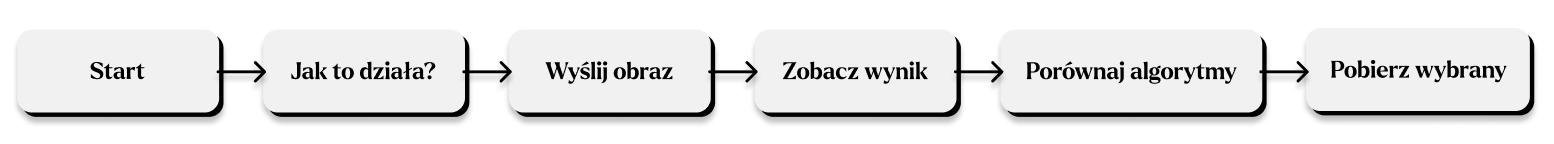
\includegraphics[width=\linewidth]{Rozdziały/06.Aplikacja/Obrazy/user-flow.png}  
        \caption{Diagram przepływu użytkownika}
        \label{fig:image82}
    \end{minipage}
\end{figure}

Diagram ten przedstawia wszystkie interakcje, które użytkownik może wykonać w aplikacji. Te interakcje nie muszą być wykorzystane, ale są dostępne dla użytkownika.

Kolejnym krokiem był projekt interfejsu użytkownika. Zdecydowałem, że narzędzie będzie składać się z dwóch ekranów: ekranu głównego \ref{fig:image80}, oraz widoku prezentacji obrazu wynikowego \ref{fig:image81}.

Projekt wyglądu aplikacji rozpocząłem od rozrysowania wireframe'ów [Rys \ref{fig:image83}] z użyciem narzędzia \textbf{Figma}, służącym do projektów graficznych między innymi aplikacji. Wireframe'y to proste szkice, które pozwalają na zobrazowanie układu elementów na stronie. Elementy te odpowiadają za funkcjonalność, a nie wygląd aplikacji i są ściśle powiązane z diagramem przepływu użytkownika.

\begin{figure}[ht]
    \centering
    \begin{minipage}[t]{0.8\linewidth}
        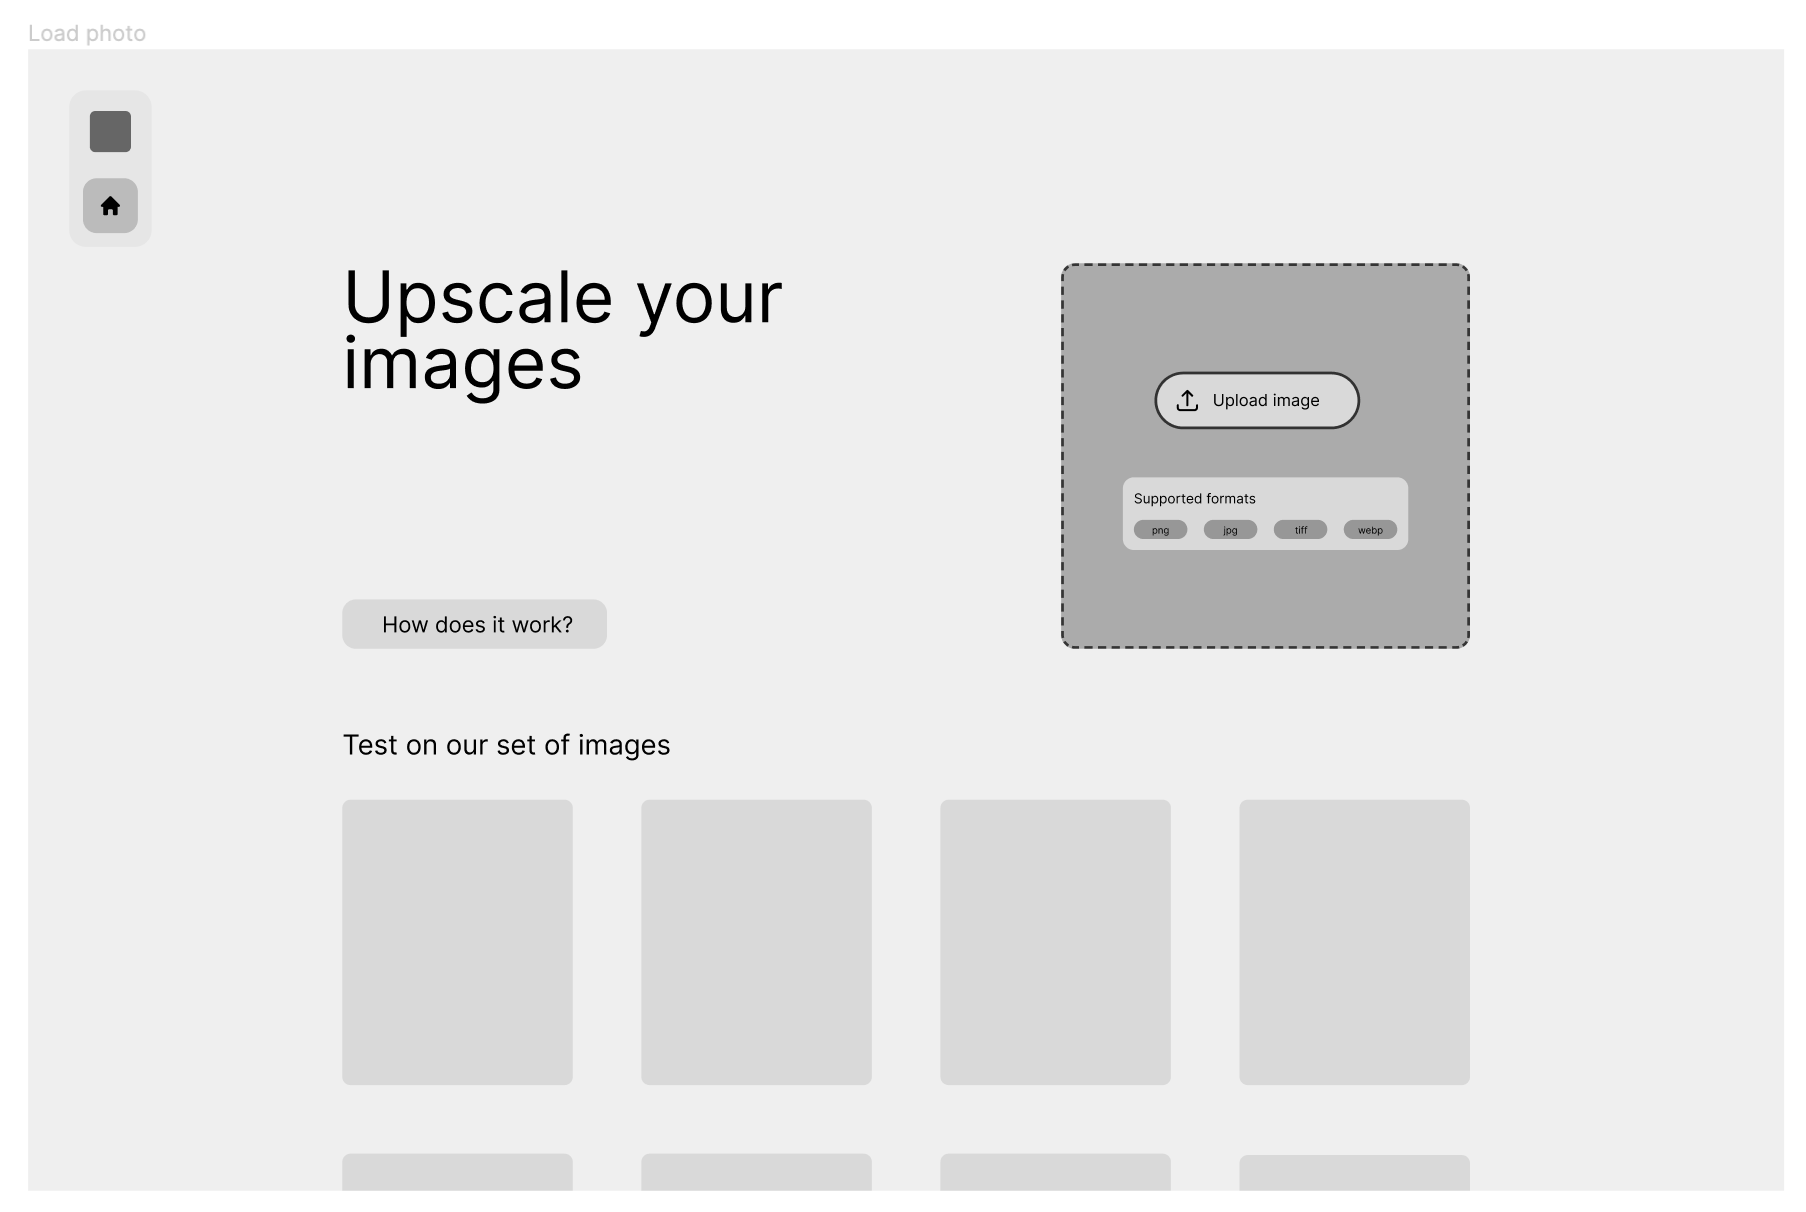
\includegraphics[width=\linewidth]{Rozdziały/06.Aplikacja/Obrazy/UX upload.png}  
        \caption{Pierwsza wersja UX aplikacji (ekran główny)}
        \label{fig:image83}
    \end{minipage}
\end{figure}

\begin{figure}[ht]
    \centering
    \begin{minipage}[t]{0.8\linewidth}
        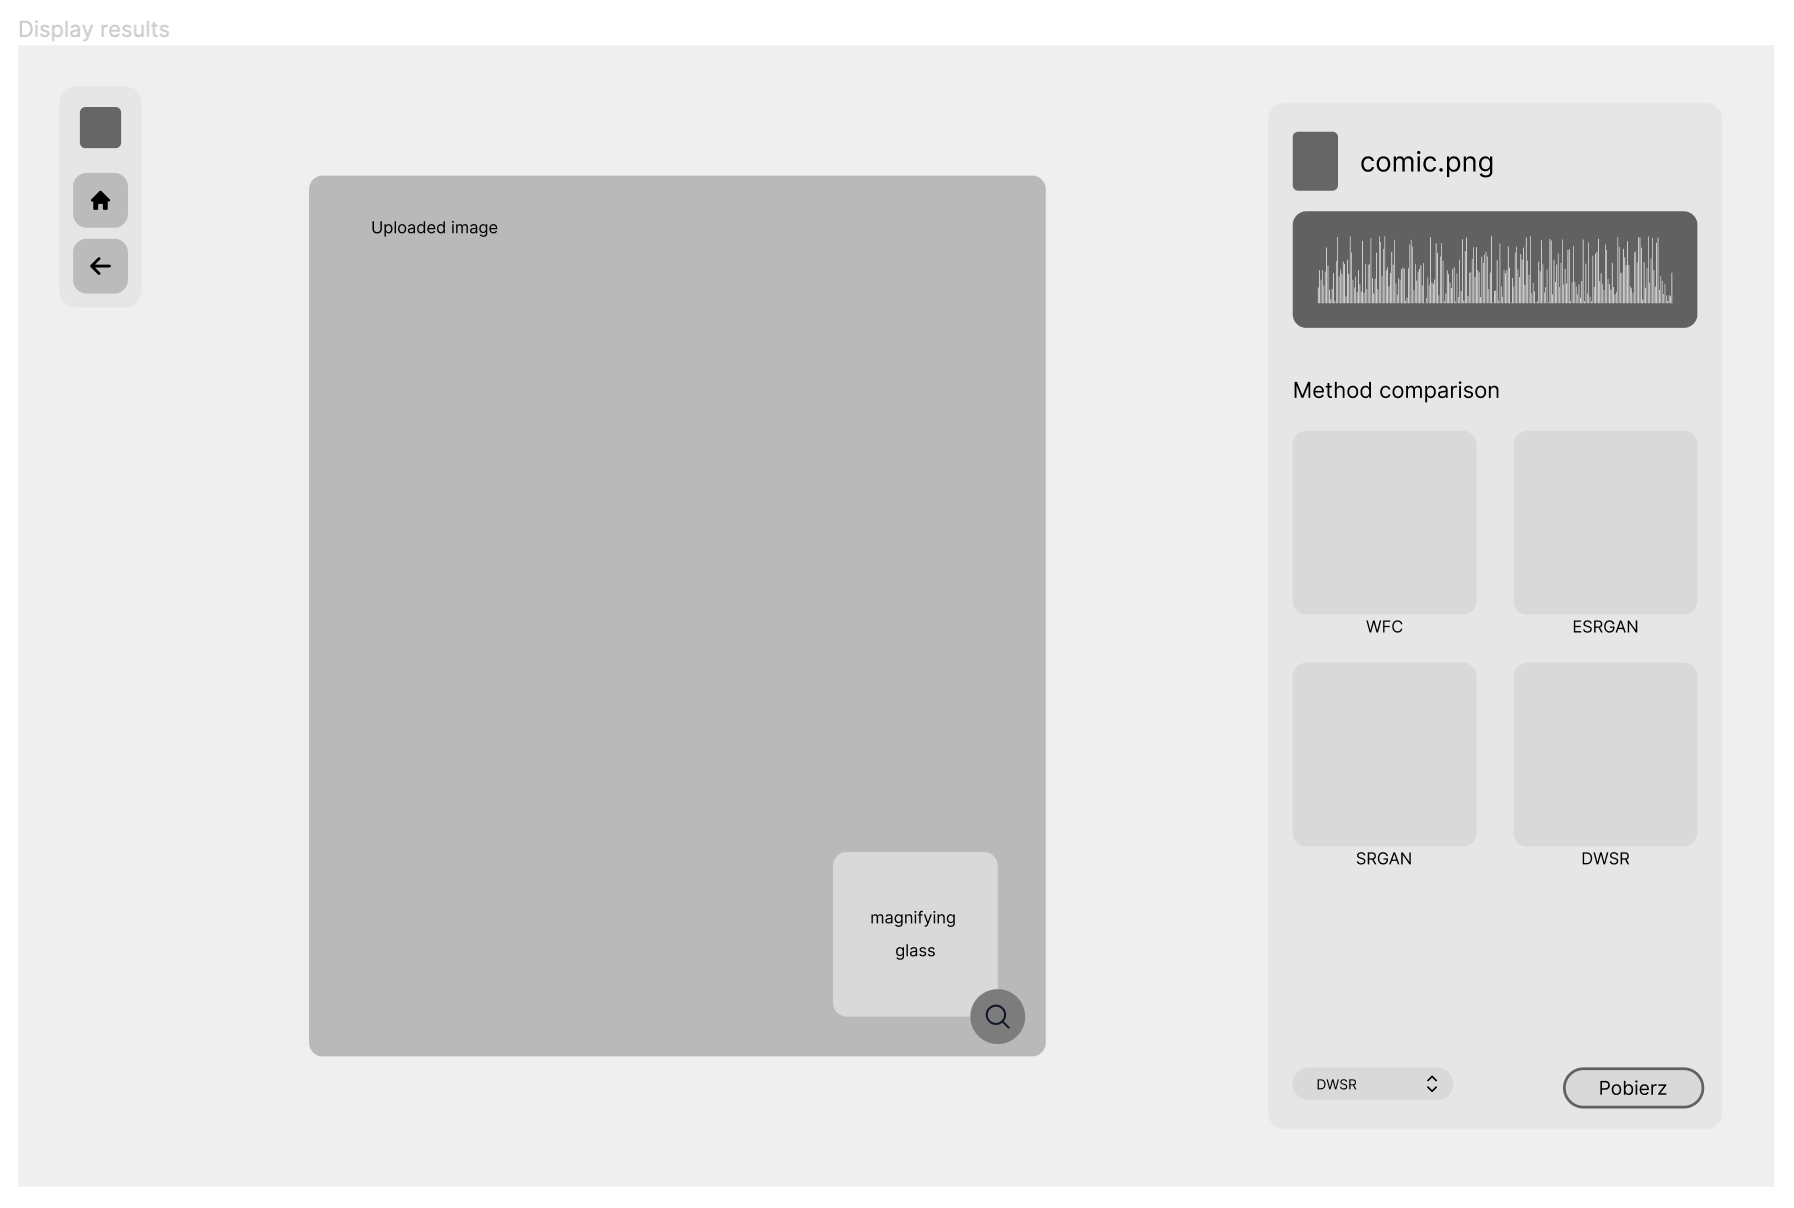
\includegraphics[width=\linewidth]{Rozdziały/06.Aplikacja/Obrazy/UX display.png}  
        \caption{Pierwsza wersja UX aplikacji (ekran prezentacji wyników)}
        \label{fig:image84}
    \end{minipage}
\end{figure}

Pierwotny rozkład elementów na stronie różni się od tego jak to wygląda teraz. Wraz z rozwojem aplikacji zmieniałem układ elementów, usprawniałem interakcję z użytkownikiem i poprawiałem rozkład elementów na ekranach aplikacji.

Kolejnym etapem pracy był projekt graficzny aplikacji. Zdecydowałem, że aplikacja będzie w ciemnym motywie, gdyż taki styl pomaga nam skupić się na tym co jest na ekranie, zwłaszcza w kontekście edycji zdjęć. Zależało mi na tym, żeby aplikacja nie była jednowymiarowa i żeby wyglądała nowocześnie. Początkowo eksperymentowałem z grafikami wektorowymi w tle [Rys \ref{fig:image85}], lecz ten wygląd nie przekonywał mnie. Eksperymentując z wyglądem pomyślałem, że w nawiązaniu do szumu na zdjęciach analogowych, tło aplikacji może mieć szum, zaś jako że mamy do czynienia z nowoczesnym narzędziem to kursor i elementy UI będą przejrzyste i czyste. W ten sposób aplikacja zyskuje na głębi i tak wygląda aktualna wersja, którą postanowiłem zaimplementować [Rys \ref{fig:image80}].
% \newpage
\begin{figure}[ht]
    \centering
    \begin{minipage}[t]{0.8\linewidth}
        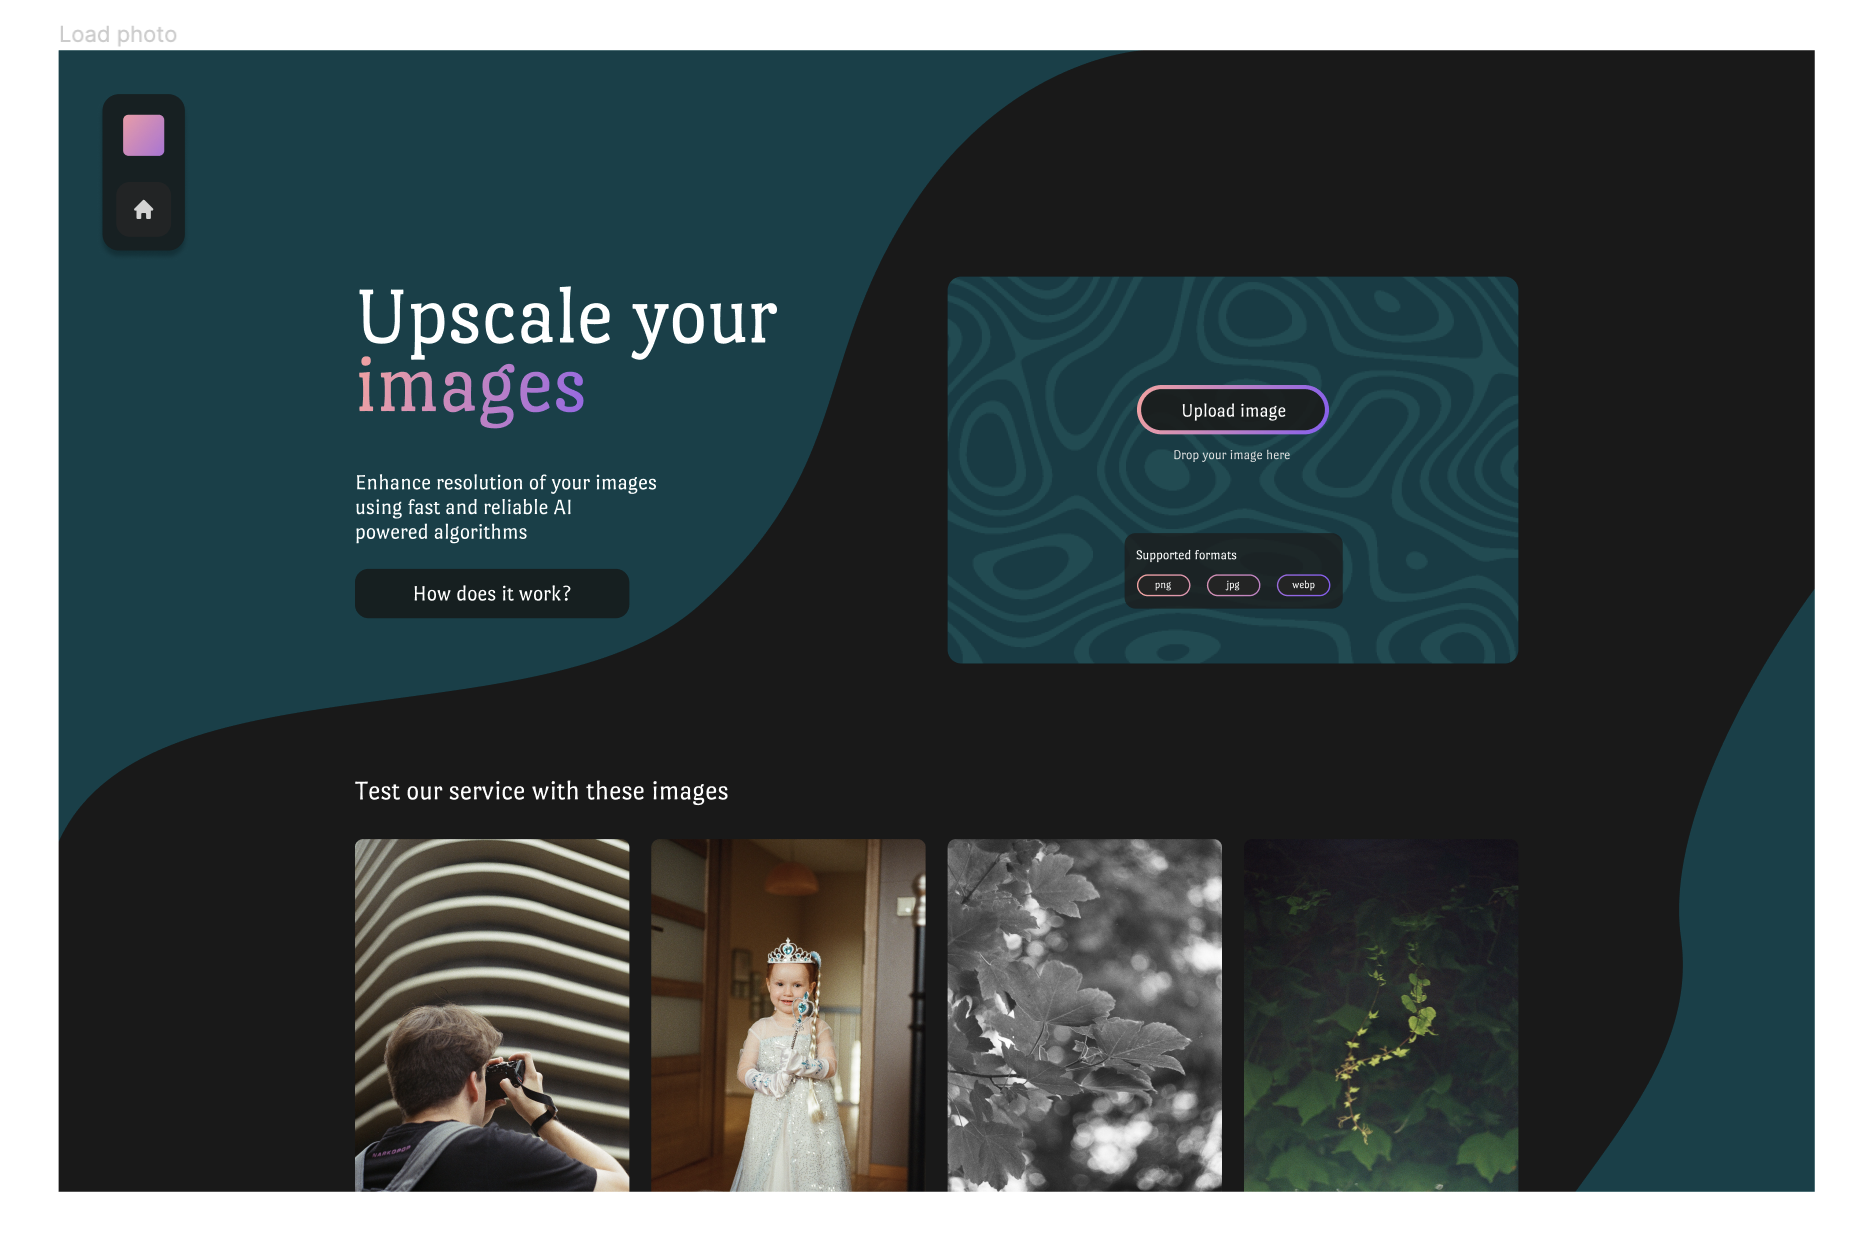
\includegraphics[width=\linewidth]{Rozdziały/06.Aplikacja/Obrazy/UI 1.png}  
        \caption{Pierwsza wersja UI strony głównej}
        \label{fig:image85}
    \end{minipage}
\end{figure}

Podobnie wyglądał proces projektowania ekranu prezentacji wyników [Rys \ref{fig:image86}]. Zdecydowałem, żeby na ekranie prezentacji wyników były tylko istotne elementy interfejsu, żeby użytkownik nie pogubił się w nadmiarze informacji. Zależało mi na tym, żeby użytkownik mógł łatwo porównać wyniki różnych algorytmów, dlatego zdecydowałem się na układ kafelków, które można wybrać i porównać z sobą. Dodatkowo w tych kafelkach uznałem, że świetnie sprawdzi się widok z bliska, który pozwoli na dokładne przyjrzenie się szczegółom obrazu, tak powstała lupka, która podąża za kursorem gdy wskaźnik znajduje się nad obrazem. 


\begin{figure}[ht]
    \centering
    \begin{minipage}[t]{0.8\linewidth}
        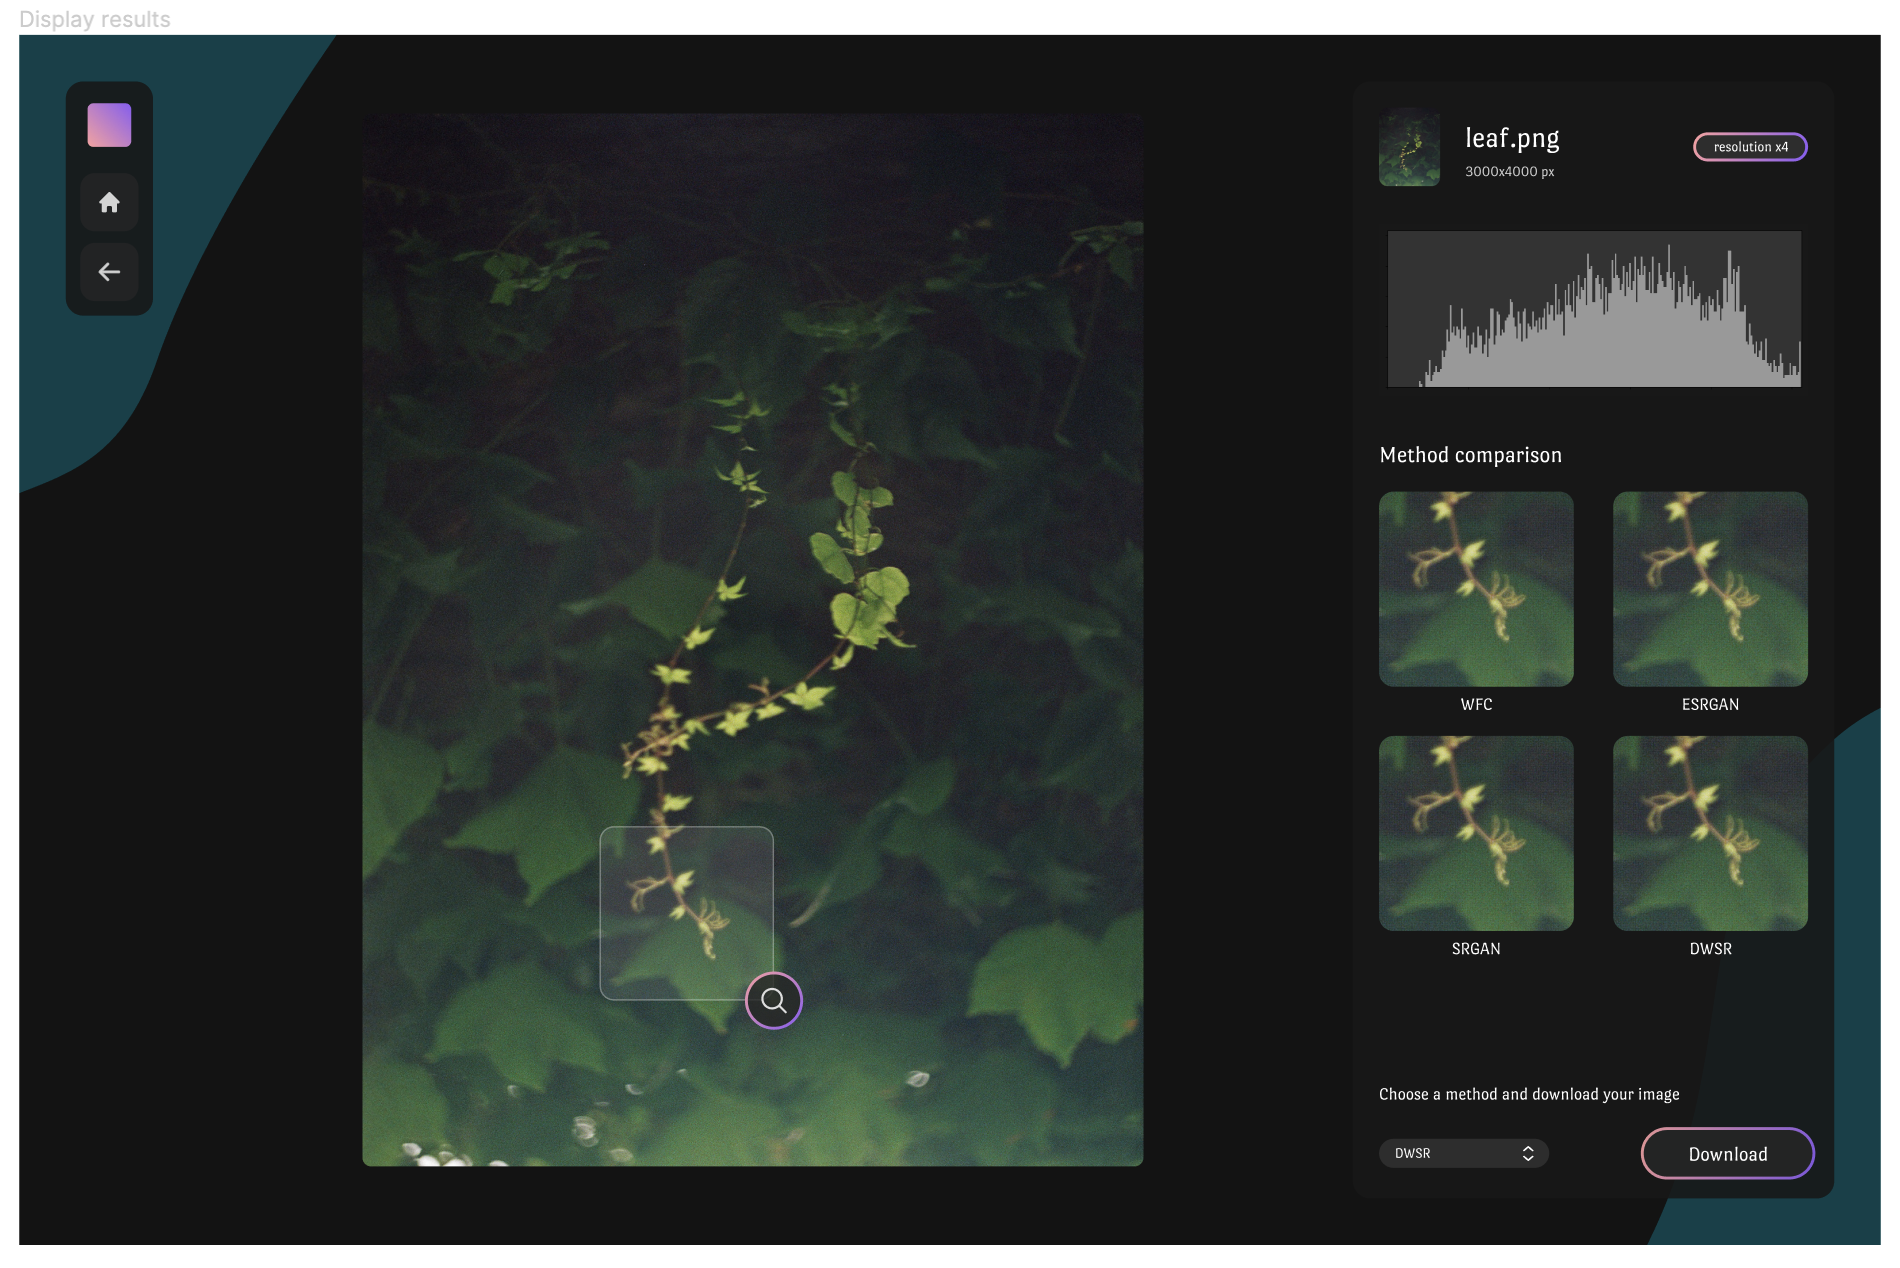
\includegraphics[width=\linewidth]{Rozdziały/06.Aplikacja/Obrazy/UI 1 dsiplay .png}  
        \caption{Pierwsza wersja UI ekranu wyświetlania wyników}
        \label{fig:image86}
    \end{minipage}
\end{figure}

W kolejnej wersji widoku prezentacji wyników postanowiłem zmienić wygląd tła. Zainspirowany aplikacjami typu \textbf{Apple Music} czy \textbf{Spotify} zdecydowałem się na zmianę tła na gradient z kolorów występujących na obrazie. W ten sposób aplikacja zyskuje na głębi i wygląda bardziej nowocześnie [Rys \ref{fig:image81}]. W tym miejscu projekt aplikacji uznałem za gotowy do implementacji. Więcej o planach rozbudowy aplikacji w rozdziale \ref{sec:plans}.



\section{Wybór narzędzi i technologii}







Wytłumaczenie wyboru określonych technologii i narzędzi użytych do stworzenia aplikacji webowej.




\section{Implementacja aplikacji}



Opis technicznego procesu integracji wybranych algorytmów z aplikacją, wraz z napotkanymi wyzwaniami.

\section{Integracja algorytmów DWSR i ESRGAN}

K-means algorytm do detekcji kolorów wystepujacych na obrazie.

\section{Wdrożenie i utrzymanie aplikacji}

Omówienie procesu wdrożenia gotowej aplikacji oraz planów dotyczących jej przyszłego utrzymania i aktualizacji.



\section{Plany na przyszłość} \label{sec:plans}

Opis błędów, rzeczy do poprawy w aplikacji. Omówienie jakie są plany rozbudowy aplikacji.